\documentclass{article}
\usepackage[utf8]{inputenc}
\usepackage[spanish]{babel}
\usepackage{listings}
\usepackage{hyperref}
\usepackage{amsmath}
\usepackage{graphicx}
\usepackage{fancyhdr}
\usepackage{geometry}
\usepackage{float}
\geometry{a4paper, margin=1in}

% Información reutilizable
\newcommand{\myTitle}{Actividad 8: Grupos de trabajo y decisiones en grupo (película Doce
hombres sin piedad)}
\newcommand{\myAuthor}{Ismael Sallami Moreno \\ Jose Ángel Carretero Montes}
\newcommand{\myDegree}{Doble Grado Ingeniería Informática y Administración y Dirección de Empresas}
\newcommand{\mySubject}{Dirección y Administración de Empresas}
\newcommand{\myDate}{\today}

\begin{document}

% Portada
\begin{titlepage}
    \centering
    \begin{minipage}{0.45\textwidth}
        \centering
        
\includegraphics[width=0.8\textwidth]{images/logo_ugr.jpg}
    \end{minipage}
    \hfill
    \begin{minipage}{0.45\textwidth}
        \centering
        
\includegraphics[width=0.8\textwidth]{images/logo_economicas.jpg} 
    \end{minipage}
    \vspace{1cm}
    
    {\scshape\LARGE \myDegree \par}
    \vspace{1cm}
    {\scshape\Large \mySubject \par}
    \vspace{1.5cm}
    {\huge\bfseries \myTitle \par}
    \vspace{2cm}
    {\Large\itshape \myAuthor \par}
    \vfill
    \myDate\par
    \vspace{2cm}
    \begin{figure}[H]
        \centering
        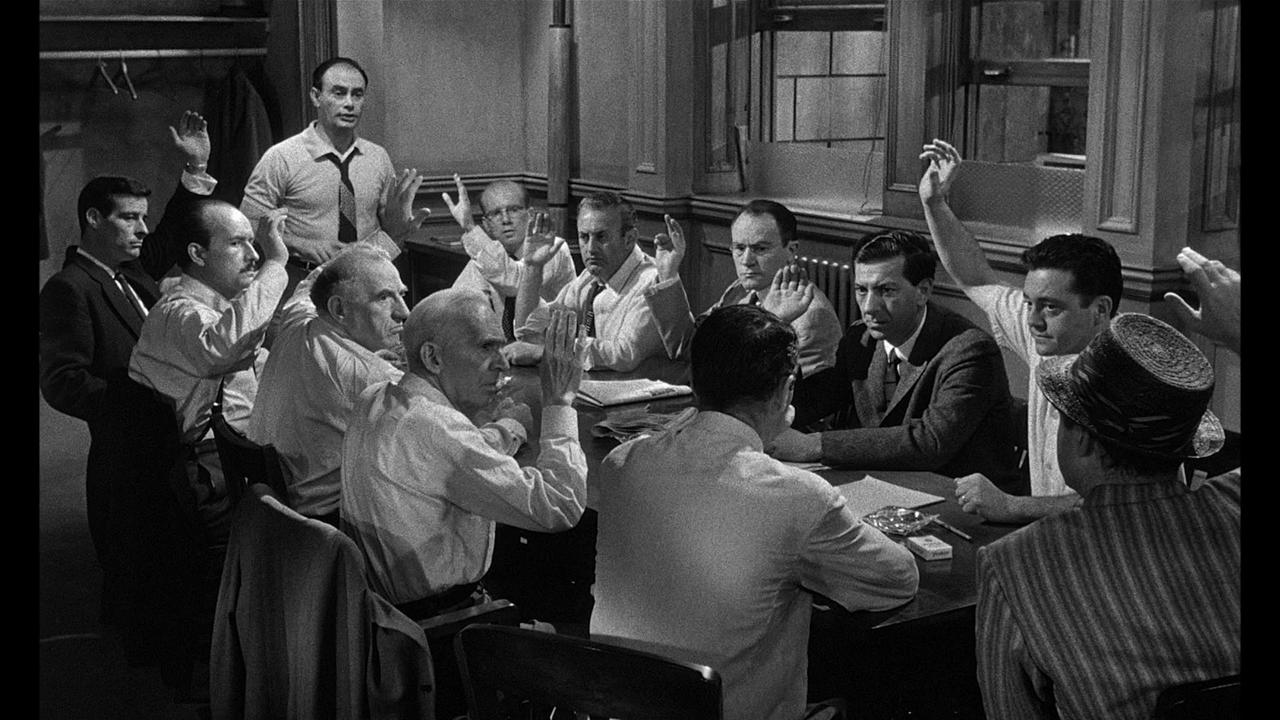
\includegraphics[width=0.7\textwidth]{images/hombres.jpeg}
    \end{figure}
\end{titlepage}

\tableofcontents
\newpage

No hay casos, en esta actividad se trata de una película

% \section{Anotaciones de la película}
% \begin{itemize}
%     \item 1: Es el presidente, es entrenador, se trata de un líder formal.
%     \item 2: Es su primera vez en un juzgado, tiene poco nerviosismo.
%     \item 3: Trabaja en correos, es muy nervioso, su hijó le pegó, menciona que va a matar al 8 y algunos de los otros hombres le exponen argumentos negativos. Relata los hechos como son, manda a callar al 2 y es un excitado.
%     \item 4: Es corredor y habla formalmente. Dice que el anciano que vió al chico lo vió corriendo hacia la puerta.La situación del chico le parece surrealista. Afirma que nunca suda, pero con las preguntas del 8 consigue sudar.
%     \item 5: Cambia su voto a inocente. Dice que el chico se ha criado con la navaja y que no la uso como saber, por eso cambia de opinión.
%     \item 6: En un principio dice que el 8 esta equivocado, vive al lado de un tren. Afirma "partirle la cara al 3 o al 4 como le hablen mal al 9."
%     \item 7: Sigue defendiendo que no saben como siguen escuchando al 8. Habla de manera informal, solo le importa ver el partido de béisbol y no muestra mucho respeto. Solo dice que le están haciendo perder el tiempo.
%     \item 8: Fiel defensor de que el chico es inocente, además de que es arquitecto.
%     \item 9: Cambia el voto a inocente, opina que el anciano que afirma haber escuchado el caso, de verdad no lo ha escuchado bien
%     \item 10: Posee gran nivel de nerviosismo y le dicen en numerosas ocasiones que se calme. Llama niño al presidente, se levanta cuando no le toca, quiere irse a trabajar en sus garajes.
%     \item 11: Les lee unas notas, piensa que el 8 dice unas declaraciones muy coherentes. Posteriormente, cambia su  voto a inocente, le piden justificación y dice que es libre de tener dudas y no tiene porque darle dicha justificación. Es educado.
%     \item 12: Él dice que si el asesinato lo hubiese cometido él, hubiese volvido a por la navaja. Aveces cuenta chistes, le parece que el problema no tiene dudas, pero luego cambian de opinión.
% \end{itemize}

% \subsection{Cronología}
% \begin{itemize}
%     \item Votan de nuevo y después comienza a llover.
%     \item Después de que varios cambien a inocente el 10 se altera y le dicen que se siente solo y no vuelva a hablar.
%     \item Comienzan a hablar sobre las marcas de las gafas y el presidente afirma que las vió en la chica, de manera que afirman que la chica quería aparentar una edad más joven.
%     \item El último que es el 3, rompe la foto y se echa a llorar, la reunión se acaba.
% \end{itemize}

% \subsection{Imagen de los personajes}
% Para ver la imagen de los personajes pincha \href{https://github.com/ElblogdeIsmael/ElblogdeIsmael.github.io/blob/main/Asignaturas/Tercer%20A%C3%B1o/DAE/PracticasDAE/ACT8/Plantilla-Practicas/images/imagenDaeAct8.pdf}{aquí.}

\section{Enunciado}

La película muestra el desarrollo de un grupo de trabajo formal (un jurado popular compuesto por 12
personas) creado por la “organización” (el tribunal de justicia) para llevar a cabo un encargo concreto.

\begin{enumerate}
    \item En primer lugar, identifique al líder formal y al líder o líderes informales. Justifique la respuesta en el caso del
    líder/es informal/es. ¿Qué otros roles o papeles aparecen desempeñados por los distintos jurados?
    \item Identifique el objetivo del grupo de trabajo y si se establecen normas de funcionamiento.
    \item Identifique en la película algunos de los factores que influyen en la cohesión de un grupo de trabajo.
    \item Analice las ventajas e inconvenientes de la toma de decisiones en grupo en comparación con las decisiones tomadas por un solo individuo (por ejemplo, si uno de los miembros del jurado fuese el encargado de hacerlo en solitario), tomando como ejemplo el proceso de decisión mostrado en la película.
    \item Por último, ¿se aprecia en la película si el grupo se ve afectado por los fenómenos de la mentalidad de grupo y giro de grupo? Si es así, ¿Cómo los superan (si es que lo hacen)?
\end{enumerate}

% \section{Respuestas de la actividad}

% \begin{enumerate}
%     \item \textbf{Identificación del líder formal e informal y otros roles en el jurado:}
    
%     El líder formal del grupo es el presidente del jurado, quien actúa como moderador y guía las discusiones. Entre los líderes informales destacan el jurado \#8, que asume un rol de defensor de la inocencia del acusado, cuestionando las evidencias presentadas. Otros roles importantes son:
%     \begin{itemize}
%         \item \textbf{Jurado \#3:} Actúa de manera dominante y conflictiva, siendo uno de los principales opositores al jurado \#8.
%         \item \textbf{Jurado \#7:} Representa la indiferencia y la falta de compromiso, interesado solo en terminar rápido para asistir a un partido.
%         \item \textbf{Jurado \#9:} Ofrece una perspectiva reflexiva y crítica hacia las evidencias, apoyando al jurado \#8 en momentos clave.
%     \end{itemize}

%     \item \textbf{Objetivo del grupo y normas de funcionamiento:}
    
%     El objetivo principal del grupo es deliberar y alcanzar un veredicto unánime sobre la culpabilidad o inocencia del acusado, basándose en las evidencias presentadas en el juicio. Aunque no se establecen normas explícitas, se espera que los miembros respeten turnos de palabra y mantengan una discusión razonada. Sin embargo, esto no siempre se cumple, generándose momentos de tensión y conflicto.

%     \item \textbf{Factores que influyen en la cohesión del grupo:}
    
%     Los factores que contribuyen a la cohesión incluyen:
%     \begin{itemize}
%         \item \textbf{Conflictos iniciales:} Aunque generan tensiones, sirven para establecer dinámicas y roles en el grupo.
%         \item \textbf{Argumentos convincentes:} Las observaciones del jurado \#8 y otros miembros logran unificar puntos de vista gradualmente.
%         \item \textbf{Empatía y reflexión:} Jurados como el \#9 fomentan la reconsideración de posturas a partir de análisis críticos.
%     \end{itemize}

%     \item \textbf{Ventajas e inconvenientes de la toma de decisiones en grupo frente a decisiones individuales:}
    
%     \begin{itemize}
%         \item \textbf{Ventajas:}
%         \begin{itemize}
%             \item Diversidad de perspectivas y análisis más detallado de las evidencias.
%             \item Mayor legitimidad en la decisión, al ser consensuada por un grupo.
%         \end{itemize}
%         \item \textbf{Inconvenientes:}
%         \begin{itemize}
%             \item Conflictos y desacuerdos que pueden retrasar el proceso.
%             \item Influencia de sesgos personales y prejuicios, dificultando la objetividad.
%         \end{itemize}
%     \end{itemize}
    
%     \item \textbf{Fenómenos de mentalidad de grupo y giro de grupo:}
    
%     En la película se observa inicialmente el fenómeno de la mentalidad de grupo, con varios jurados inclinándose hacia la culpabilidad sin cuestionar las evidencias. Sin embargo, gracias a las intervenciones del jurado \#8, se supera este problema mediante análisis críticos y argumentos sólidos. En cuanto al giro de grupo, se aprecia un cambio hacia una posición más reflexiva y unificada, resultado de las discusiones y el intercambio de ideas.
% \end{enumerate}

\section{Respuestas de la actividad }
\subsection{Identificación del líder formal e informal y otros roles en el jurado}

El líder formal es aquel designado oficialmente como responsable de un grupo, equipo o proyecto. En el caso de la película, el jurado número 1 cumple este rol, encargándose de mantener el orden y asegurando que el proceso de deliberación se lleve a cabo de manera organizada y efectiva. 

Sin embargo, a lo largo de la película surgen líderes informales, individuos que, sin un nombramiento oficial, influyen significativamente en las dinámicas del grupo y en las opiniones de sus miembros:

\begin{itemize}
    \item \textbf{El jurado número 8:} Inicialmente, se muestra en desacuerdo con la mayoría al expresar dudas sobre la culpabilidad del acusado. A medida que avanza la deliberación, sus argumentos convincentes lo posicionan como un líder informal, logrando que otros jurados reconsideren sus decisiones iniciales.
    \item \textbf{El jurado número 3:} Desde el inicio, adopta una postura firme a favor de la culpabilidad del acusado. Su actitud dominante y persistencia en defender esta postura también lo convierten en un líder informal dentro del grupo.
\end{itemize}

Además de los líderes formales e informales, se pueden identificar otros roles entre los miembros del jurado:

\begin{itemize}
    \item \textbf{Rol de especialista en tareas:} Miembros que dedican tiempo y esfuerzo a apoyar al grupo en la consecución de su objetivo. 
    \item \textbf{Rol socioemocional:} Aquellos que se centran en satisfacer las necesidades emocionales de los integrantes del grupo y en fortalecer la cohesión social.
    \item \textbf{Rol no participativo o disfuncional:} Personas que contribuyen poco al proceso de deliberación y en ocasiones dificultan el avance del grupo.
\end{itemize}

A continuación, le adjuntamos una imagen en la que figuran los jurados según los roles identificados.
\newpage
\begin{figure}[H]
    \centering
    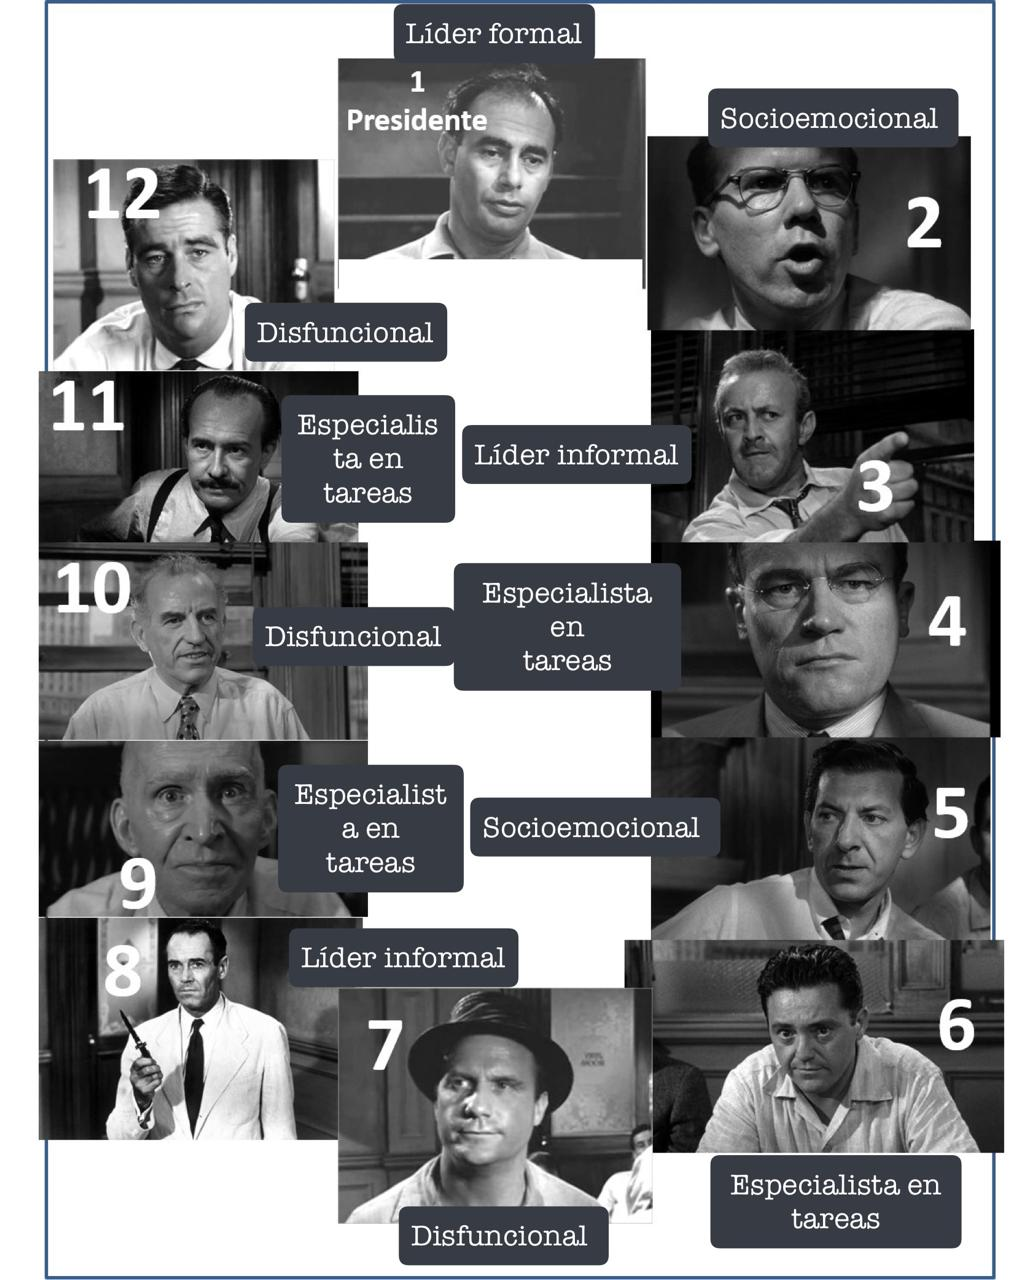
\includegraphics[width=0.8\textwidth]{images/jurado.jpeg}
    \caption{Roles identificados en el jurado de la película.}
    \label{fig:roles_jurado}
\end{figure}
\newpage

\subsection{Identificación del objetivo del grupo de trabajo y si se establecen normas de funcionamiento}

El propósito principal del grupo de trabajo es deliberar y llegar a un acuerdo unánime sobre la culpabilidad o inocencia del acusado, un joven señalado por asesinato en primer grado. Esta decisión es crucial, ya que determinará si el acusado será condenado a la silla eléctrica o absuelto. Para ello, los 12 miembros del jurado se reúnen en una sala para llevar a cabo el proceso de deliberación.\\

Existen normas que regulan el funcionamiento del grupo, con el objetivo de establecer un marco de comportamiento aceptable y garantizar que se cumpla con la tarea asignada. Estas normas incluyen diversos puntos que vamos a detallar a continuación.
La decisión final debe ser unánime, como lo estipula la ley. Todos los miembros deben estar presentes para iniciar la deliberación y las votaciones deben realizarse de manera formal. Se deben respetar los turnos de palabra, permitiendo que cada miembro exprese sus opiniones. Es fundamental que los jurados mantengan el respeto mutuo, independientemente de las diferencias en sus puntos de vista. Existe un límite de tiempo para alcanzar una decisión; si no es posible, se informará al juez de la falta de consenso. Los jurados deben mantenerse enfocados en el objetivo, evitando discusiones irrelevantes.

\subsection{Identificación de factores que influyen en la cohesión de un grupo de trabajo}

La cohesión en un grupo de trabajo es un elemento clave que puede modificar tanto las actitudes como los comportamientos de sus integrantes. En la película se identifican diversos factores que influyen positiva y negativamente en este aspecto:

\begin{itemize}
    \item \textbf{Tamaño del grupo:} El jurado está compuesto por 12 personas, lo cual representa un grupo relativamente grande. Esto puede dificultar la comunicación y la búsqueda de consenso debido a la cantidad de opiniones diversas.
    
    \item \textbf{Diversidad:} Aunque la mayoría de los miembros del jurado pertenecen al mismo rango de edad, provienen de distintos contextos sociales y ejercen profesiones variadas, como publicistas, empresarios, pintores y arquitectos. Estas diferencias enriquecen las discusiones, pero también generan conflictos debido a la dificultad de encontrar puntos de vista comunes.

    \item \textbf{Competencia sana:} La ausencia de una competencia saludable afecta negativamente la cohesión del grupo. Durante la película, se observan episodios de confrontaciones personales, amenazas e insultos cuando los jurados no comparten opiniones similares, lo que obstaculiza un ambiente constructivo.

    \item \textbf{Éxito grupal:} El objetivo principal del jurado era alcanzar un veredicto unánime. A pesar de las diferencias iniciales y los conflictos, el grupo logró superar las discrepancias y llegar a un consenso final, lo que demuestra un grado de éxito en su cohesión.

    \item \textbf{Grado de interacción:} La interacción entre los miembros del jurado es alta, con la mayoría de ellos participando activamente en las deliberaciones y expresando sus opiniones. Sin embargo, algunos jurados, como el número 7, afectan negativamente la cohesión grupal debido al comportamiento que desempeñan.

    \item \textbf{Objetivos compartidos:} En un principio, no todos los miembros compartían el objetivo común de deliberar cuidadosamente. Mientras algunos deseaban resolver el caso de manera rápida, otros estaban comprometidos con analizar las evidencias en profundidad. Esta disparidad inicial dificultó la cohesión, aunque finalmente se alinearon hacia un propósito común.

    \item \textbf{Atracción interpersonal:} La cohesión del grupo también se ve afectada por las relaciones interpersonales. Las tensiones y confrontaciones observadas, como insultos y amenazas, debilitaron temporalmente la unión del grupo, aunque estos conflictos se resolvieron a medida que avanzaba la deliberación.
\end{itemize}

\subsection{Análisis de las ventajas e inconvenientes de la toma de decisiones en grupo frente a decisiones individuales}

\begin{itemize}
    \item La toma de decisiones en grupo presenta diversas \textbf{ventajas} significativas. En primer lugar, permite incorporar una variedad de perspectivas, lo que facilita un análisis más completo del problema desde diferentes ángulos. Esto, a su vez, enriquece el conocimiento colectivo y conduce a decisiones más informadas y justas. Además, la participación activa de la mayoría de los integrantes fomenta un mayor compromiso con el resultado final. Otra ventaja destacable es la mitigación de sesgos individuales, ya que la diversidad de opiniones contribuye a equilibrar puntos de vista y promover objetividad.
    \item También existen \textbf{desventajas} asociadas a este tipo de decisiones. Los conflictos y tensiones entre los miembros, derivados de diferencias de opinión, pueden generar un ambiente hostil. Asimismo, la presión por conformarse con la mayoría puede influir negativamente en las votaciones, como se observa al inicio de la película, cuando varios jurados optan por declarar culpable al acusado sin expresar sus verdaderas opiniones. Otra desventaja es la influencia desproporcionada de personalidades dominantes como es el caso de los personajes del jurado 3 y 8, que pueden inclinar el debate hacia sus propias posturas, como ocurre en las primeras etapas de la deliberación. Además, la polarización dentro del grupo dificulta alcanzar un consenso, dando lugar a posiciones diametralmente opuestas. También es común la tendencia hacia decisiones percibidas como menos arriesgadas, como la inclinación inicial hacia la culpabilidad del acusado, y la falta de responsabilidad individual, ejemplificada claramente en la actitud del jurado número 7, quien muestra desinterés por el proceso.

\end{itemize}

\subsection{Fenómenos de mentalidad de grupo y giro de grupo}

En la película y según la teoría, se pueden observar claramente los fenómenos de la mentalidad de grupo y el giro de grupo, los cuales se manifiestan a medida que avanza la trama.

La \textbf{mentalidad de grupo} es un fenómeno psicológico que ocurre cuando el deseo de conformidad y de mantener la armonía dentro del grupo prevalece sobre el juicio individual y la toma de decisiones críticas. Este fenómeno es evidente al principio de la película, cuando algunos miembros del jurado sienten una fuerte presión por llegar a un veredicto rápido y unánime, con el fin de retomar sus actividades personales. En este contexto, varios jurados se conforman con la opinión predominante sin cuestionarla. Además, la influencia de personalidades dominantes también afecta el proceso, ya que la tendencia a seguir al líder de grupo distorsiona las percepciones y decisiones de los demás miembros.

Por otro lado, el \textbf{giro de grupo} se refiere al cambio de opiniones que experimentan los miembros del grupo después de un proceso de deliberación. A lo largo de la película, algunos jurados modifican su postura inicial debido a la presentación de nuevos argumentos y pruebas que cuestionan sus primeras percepciones. A medida que avanza la deliberación, varios miembros del jurado desafían la conformidad inicial, planteando dudas, cuestionando las evidencias presentadas y ofreciendo nuevas interpretaciones de los hechos.

Para superar estos fenómenos, el diálogo y el debate son fundamentales, ya que permiten que los jurados reconsideren sus opiniones a partir de nuevas interpretaciones de la evidencia. Es esencial realizar un análisis crítico de la información disponible, revisando detalladamente los testimonios y reconstruyendo los hechos de manera objetiva. Además, es necesario que los miembros del jurado desarrollen empatía y comprensión mutua. A lo largo de la película, se observa un creciente entendimiento entre los jurados, lo que contribuye a superar la presión de la conformidad y facilita la toma de una decisión colectiva más reflexiva y equilibrada.








\end{document}